%%
%% Automatically generated file from DocOnce source
%% (https://github.com/hplgit/doconce/)
%%
%%
% #ifdef PTEX2TEX_EXPLANATION
%%
%% The file follows the ptex2tex extended LaTeX format, see
%% ptex2tex: http://code.google.com/p/ptex2tex/
%%
%% Run
%%      ptex2tex myfile
%% or
%%      doconce ptex2tex myfile
%%
%% to turn myfile.p.tex into an ordinary LaTeX file myfile.tex.
%% (The ptex2tex program: http://code.google.com/p/ptex2tex)
%% Many preprocess options can be added to ptex2tex or doconce ptex2tex
%%
%%      ptex2tex -DMINTED myfile
%%      doconce ptex2tex myfile envir=minted
%%
%% ptex2tex will typeset code environments according to a global or local
%% .ptex2tex.cfg configure file. doconce ptex2tex will typeset code
%% according to options on the command line (just type doconce ptex2tex to
%% see examples). If doconce ptex2tex has envir=minted, it enables the
%% minted style without needing -DMINTED.
% #endif

% #define PREAMBLE

% #ifdef PREAMBLE
%-------------------- begin preamble ----------------------

\documentclass[%
oneside,                 % oneside: electronic viewing, twoside: printing
final,                   % draft: marks overfull hboxes, figures with paths
10pt]{article}

\listfiles               %  print all files needed to compile this document

\usepackage{relsize,makeidx,color,setspace,amsmath,amsfonts,amssymb}
\usepackage[table]{xcolor}
\usepackage{bm,ltablex,microtype}

\usepackage[pdftex]{graphicx}

\usepackage[T1]{fontenc}
%\usepackage[latin1]{inputenc}
\usepackage{ucs}
\usepackage[utf8x]{inputenc}

\usepackage{lmodern}         % Latin Modern fonts derived from Computer Modern

% Hyperlinks in PDF:
\definecolor{linkcolor}{rgb}{0,0,0.4}
\usepackage{hyperref}
\hypersetup{
    breaklinks=true,
    colorlinks=true,
    linkcolor=linkcolor,
    urlcolor=linkcolor,
    citecolor=black,
    filecolor=black,
    %filecolor=blue,
    pdfmenubar=true,
    pdftoolbar=true,
    bookmarksdepth=3   % Uncomment (and tweak) for PDF bookmarks with more levels than the TOC
    }
%\hyperbaseurl{}   % hyperlinks are relative to this root

\setcounter{tocdepth}{2}  % levels in table of contents

% Tricks for having figures close to where they are defined:
% 1. define less restrictive rules for where to put figures
\setcounter{topnumber}{2}
\setcounter{bottomnumber}{2}
\setcounter{totalnumber}{4}
\renewcommand{\topfraction}{0.95}
\renewcommand{\bottomfraction}{0.95}
\renewcommand{\textfraction}{0}
\renewcommand{\floatpagefraction}{0.75}
% floatpagefraction must always be less than topfraction!
% 2. ensure all figures are flushed before next section
\usepackage[section]{placeins}
% 3. enable begin{figure}[H] (often leads to ugly pagebreaks)
%\usepackage{float}\restylefloat{figure}

% prevent orhpans and widows
\clubpenalty = 10000
\widowpenalty = 10000

\newenvironment{doconceexercise}{}{}
\newcounter{doconceexercisecounter}


% ------ header in subexercises ------
%\newcommand{\subex}[1]{\paragraph{#1}}
%\newcommand{\subex}[1]{\par\vspace{1.7mm}\noindent{\bf #1}\ \ }
\makeatletter
% 1.5ex is the spacing above the header, 0.5em the spacing after subex title
\newcommand\subex{\@startsection{paragraph}{4}{\z@}%
                  {1.5ex\@plus1ex \@minus.2ex}%
                  {-0.5em}%
                  {\normalfont\normalsize\bfseries}}
\makeatother


% --- end of standard preamble for documents ---


% insert custom LaTeX commands...

\raggedbottom
\makeindex
\usepackage[totoc]{idxlayout}   % for index in the toc
\usepackage[nottoc]{tocbibind}  % for references/bibliography in the toc

%-------------------- end preamble ----------------------

\begin{document}

% matching end for #ifdef PREAMBLE
% #endif

\newcommand{\exercisesection}[1]{\subsection*{#1}}


% ------------------- main content ----------------------



% ----------------- title -------------------------

\thispagestyle{empty}

\begin{center}
{\LARGE\bf
\begin{spacing}{1.25}
FFM234, Klassisk fysik och vektorfält - Veckans tal
\end{spacing}
}
\end{center}

% ----------------- author(s) -------------------------

\begin{center}
{\bf Christin Rhen, Chalmers${}^{}$} \\ [0mm]
\end{center}

\begin{center}
% List of all institutions:
\end{center}
    
% ----------------- end author(s) -------------------------

% --- begin date ---
\begin{center}
Aug 10, 2019
\end{center}
% --- end date ---

\vspace{1cm}


% --- begin exercise ---
\begin{doconceexercise}
\refstepcounter{doconceexercisecounter}

\subsection{Uppgift 7.5.1: Stegfunktioner och deltafunktioner}

Konstruera approximationerna till stegfunktionen svarande mot approximationerna av deltafunktionen i ekv. (7.6), (7.7) och (7.8)!

% --- begin hint in exercise ---

\paragraph{Hint.}
\begin{itemize}
\item Varje given deltafunktions-approximation kan integreras och ger då en motsvarande stegfunktions-approximation. 

\item Utför integralen först och låt sedan $\epsilon \to 0$. Glöm inte att skissa funktionerna.

\item I fallet med den Gaussiska deltafunktions-approximationen får man en primitiv funktion som innehåller den s.k. felfunktionen $\mathrm{erf}(x)$.
\end{itemize}

\noindent
% --- end hint in exercise ---


% --- begin answer of exercise ---
\paragraph{Answer.}
I samtliga fall har man $\sigma_\epsilon (x)=\int_{-\infty}^x h_\epsilon (y)dy$, där $h_\epsilon(x)$ är approximationen av $\delta(x)$. Svarande mot (7.6) har man en styckvis linjär och kontinuerlig funktion som är 0 för $x<-\frac{\epsilon}{2}$, 1 för $x>\frac{\epsilon}{2}$ och växer linjärt däremellan. Svarande mot (7.7) har man $\sigma_\epsilon(x)=\frac{1}{2}\left(1+\mathrm{erf}(\frac{x}{\epsilon})\right)$ och mot (7.8) har man $\sigma_\epsilon(x)=\frac{1}{2}+\frac{1}{\pi}\tanh(\frac{x}{\epsilon})$.

% --- end answer of exercise ---


% --- begin solution of exercise ---
\paragraph{Solution.}
Stegfunktionen kan definieras som (ekvation (7.10) i kurskompendiet)
\begin{equation}
    H(x) =\int_{-\infty}^x\mathrm dt\ \delta(t)=\left\{\begin{array}{cc}
        0 & x < 0 \\
        1 & x > 0
    \end{array} \right..
    \label{step}
\end{equation}
Exakt vilket värde $H(0)$ antar varierar i litteraturen. Vanligt är att $H(0)$ är odefinierat eller lika med $1/2$. 

Varje given deltafunktions-approximation kan alltså integreras enligt ekvation~(\ref{step}) och ger då en motsvarande stegfunktions-approximation. Till exempel kan
\begin{equation}
    \delta(x)=\lim_{\epsilon\rightarrow 0}h_\epsilon(x) =\lim_{\epsilon\rightarrow 0}\left\{\begin{array}{cc}
        1/\epsilon & |x| < \epsilon/2 \\
        0 & |x| > \epsilon/2
    \end{array} \right.
\end{equation}
integreras trivialt till (med eget val av integrationskonstant)
\begin{equation}
    H(x)=\lim_{\epsilon\rightarrow 0}\left\{\begin{array}{cc}
        0 & x < -\epsilon/2 \\
        \frac{x}{\epsilon}+\frac{1}{2} & -\epsilon/2<x<\epsilon/2 \\
        1 & x > \epsilon/2
    \end{array} \right..
\end{equation}

För den Gaussiska deltafunktions-approximationen $h_\epsilon(x) =\exp\left[-x^2/\epsilon^2\right]/\epsilon\sqrt\pi$ får vi stegfunktionen (med eget val av integrationskonstant)
\begin{equation}
H(x)=\lim_{\epsilon\rightarrow 0}\frac{1}{2}\left[1+\mathrm{erf}\left(\frac{ x}{\epsilon}\right)\right].
\end{equation}
Här är felfunktionen
\begin{equation}
    \mathrm{erf}(x)=\frac2{\sqrt\pi}\int_0^x\mathrm dt\ e^{-t^2}.
\end{equation}

Slutligen har vi den Lorentzianska approximationen $h_\epsilon(x)=\epsilon\pi^{-1}(x^2+\epsilon^2)^{-1}$, som även den är rättfram att integrera. Resultatet är (med eget val av integrationskonstant)
\begin{equation}
H(x)=\lim_{\epsilon\rightarrow 0}\left[\tfrac12+\tfrac12\tanh\left(\tfrac x\epsilon\right)\right].
\end{equation}

Utseendet på dessa funktioner skissas i figurerna~\ref{fig:711} och~\ref{fig:712} för några olika värden på $\epsilon$.


\begin{figure}[!ht]  % fig:711
  \centerline{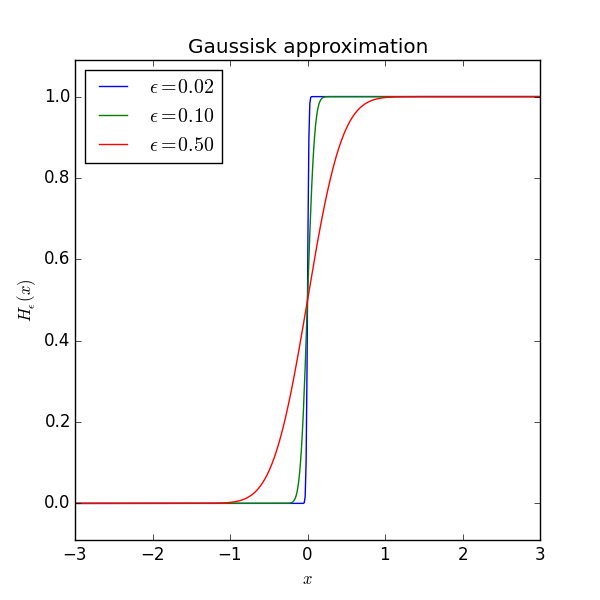
\includegraphics[width=0.6\linewidth]{fig/fig711.png}}
  \caption{
  Primitiva funktionen till den Gaussiska approximationen av deltafunktionen i gränsen $\epsilon \to 0$. \label{fig:711}
  }
\end{figure}
%\clearpage % flush figures fig:711



\begin{figure}[!ht]  % fig:712
  \centerline{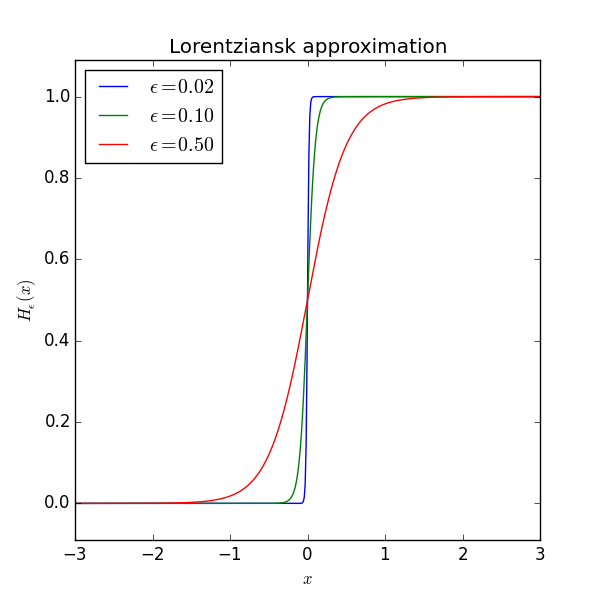
\includegraphics[width=0.6\linewidth]{fig/fig712.png}}
  \caption{
  Primitiva funktionen till den Lorentziska approximationen av deltafunktionen i gränsen $\epsilon \to 0$. \label{fig:712}
  }
\end{figure}
%\clearpage % flush figures fig:712


% --- end solution of exercise ---

% Closing remarks for this Exercise

\paragraph{Remarks.}
Uppgiften illustrerar hur en stegfunktion resulterar som en primitiv funktion till en deltafunktion. Vi undersöker olika distributioner för vilka integralen kan utföras analytiskt och studerar sedan gränsen då $\epsilon \to 0$.


\end{doconceexercise}
% --- end exercise ---


% ------------------- end of main content ---------------

% #ifdef PREAMBLE
\end{document}
% #endif

